% Options for packages loaded elsewhere
\PassOptionsToPackage{unicode}{hyperref}
\PassOptionsToPackage{hyphens}{url}
%
\documentclass[
  ignorenonframetext,
  aspectratio=169]{beamer}
\usepackage{pgfpages}
\setbeamertemplate{caption}[numbered]
\setbeamertemplate{caption label separator}{: }
\setbeamercolor{caption name}{fg=normal text.fg}
\beamertemplatenavigationsymbolsempty
% Prevent slide breaks in the middle of a paragraph
\widowpenalties 1 10000
\raggedbottom
\setbeamertemplate{part page}{
  \centering
  \begin{beamercolorbox}[sep=16pt,center]{part title}
    \usebeamerfont{part title}\insertpart\par
  \end{beamercolorbox}
}
\setbeamertemplate{section page}{
  \centering
  \begin{beamercolorbox}[sep=12pt,center]{part title}
    \usebeamerfont{section title}\insertsection\par
  \end{beamercolorbox}
}
\setbeamertemplate{subsection page}{
  \centering
  \begin{beamercolorbox}[sep=8pt,center]{part title}
    \usebeamerfont{subsection title}\insertsubsection\par
  \end{beamercolorbox}
}
\AtBeginPart{
  \frame{\partpage}
}
\AtBeginSection{
  \ifbibliography
  \else
    \frame{\sectionpage}
  \fi
}
\AtBeginSubsection{
  \frame{\subsectionpage}
}
\usepackage{amsmath,amssymb}
\usepackage{lmodern}
\usepackage{iftex}
\ifPDFTeX
  \usepackage[T1]{fontenc}
  \usepackage[utf8]{inputenc}
  \usepackage{textcomp} % provide euro and other symbols
\else % if luatex or xetex
  \usepackage{unicode-math}
  \defaultfontfeatures{Scale=MatchLowercase}
  \defaultfontfeatures[\rmfamily]{Ligatures=TeX,Scale=1}
\fi
\usetheme[]{Szeged}
\usecolortheme{spruce}
% Use upquote if available, for straight quotes in verbatim environments
\IfFileExists{upquote.sty}{\usepackage{upquote}}{}
\IfFileExists{microtype.sty}{% use microtype if available
  \usepackage[]{microtype}
  \UseMicrotypeSet[protrusion]{basicmath} % disable protrusion for tt fonts
}{}
\makeatletter
\@ifundefined{KOMAClassName}{% if non-KOMA class
  \IfFileExists{parskip.sty}{%
    \usepackage{parskip}
  }{% else
    \setlength{\parindent}{0pt}
    \setlength{\parskip}{6pt plus 2pt minus 1pt}}
}{% if KOMA class
  \KOMAoptions{parskip=half}}
\makeatother
\usepackage{xcolor}
\IfFileExists{xurl.sty}{\usepackage{xurl}}{} % add URL line breaks if available
\IfFileExists{bookmark.sty}{\usepackage{bookmark}}{\usepackage{hyperref}}
\hypersetup{
  pdftitle={Spike-and-Slab Additive Models And Fast Algorithms For High-Dimensional Data Analysis},
  pdfauthor={Boyi Guo},
  hidelinks,
  pdfcreator={LaTeX via pandoc}}
\urlstyle{same} % disable monospaced font for URLs
\newif\ifbibliography
\usepackage{graphicx}
\makeatletter
\def\maxwidth{\ifdim\Gin@nat@width>\linewidth\linewidth\else\Gin@nat@width\fi}
\def\maxheight{\ifdim\Gin@nat@height>\textheight\textheight\else\Gin@nat@height\fi}
\makeatother
% Scale images if necessary, so that they will not overflow the page
% margins by default, and it is still possible to overwrite the defaults
% using explicit options in \includegraphics[width, height, ...]{}
\setkeys{Gin}{width=\maxwidth,height=\maxheight,keepaspectratio}
% Set default figure placement to htbp
\makeatletter
\def\fps@figure{htbp}
\makeatother
\setlength{\emergencystretch}{3em} % prevent overfull lines
\providecommand{\tightlist}{%
  \setlength{\itemsep}{0pt}\setlength{\parskip}{0pt}}
\setcounter{secnumdepth}{-\maxdimen} % remove section numbering
\newlength{\cslhangindent}
\setlength{\cslhangindent}{1.5em}
\newlength{\csllabelwidth}
\setlength{\csllabelwidth}{3em}
\newlength{\cslentryspacingunit} % times entry-spacing
\setlength{\cslentryspacingunit}{\parskip}
\newenvironment{CSLReferences}[2] % #1 hanging-ident, #2 entry spacing
 {% don't indent paragraphs
  \setlength{\parindent}{0pt}
  % turn on hanging indent if param 1 is 1
  \ifodd #1
  \let\oldpar\par
  \def\par{\hangindent=\cslhangindent\oldpar}
  \fi
  % set entry spacing
  \setlength{\parskip}{#2\cslentryspacingunit}
 }%
 {}
\usepackage{calc}
\newcommand{\CSLBlock}[1]{#1\hfill\break}
\newcommand{\CSLLeftMargin}[1]{\parbox[t]{\csllabelwidth}{#1}}
\newcommand{\CSLRightInline}[1]{\parbox[t]{\linewidth - \csllabelwidth}{#1}\break}
\newcommand{\CSLIndent}[1]{\hspace{\cslhangindent}#1}
\usepackage{amsmath}
\usepackage{tikz}
\usepackage{pgfplots}
\usepackage{bm}
\usetikzlibrary{shapes.geometric, arrows, positioning, calc, matrix, backgrounds, fit}
\newcommand{\bs}[1]{\boldsymbol{#1}}
\newcommand{\tp}{*}
\newcommand{\pr}{\text{Pr}}
\newcommand{\repa}{\text{repa}}
\newcommand{\simiid}{\overset{\text{iid}}{\sim}}
\newcommand{\bg}[1]{\textcolor{red}{#1}}
\ifLuaTeX
  \usepackage{selnolig}  % disable illegal ligatures
\fi

\title{Spike-and-Slab Additive Models And Fast Algorithms For
High-Dimensional Data Analysis}
\author{Boyi Guo}
\date{July 12th, 2022}
\institute{Department of Biostatistics\\
University of Alabama at Birmingham}

\begin{document}
\frame{\titlepage}

\hypertarget{outline}{%
\section*{Outline}\label{outline}}

\begin{frame}{Outline}
\begin{itemize}
\tightlist
\item
  Background

  \begin{itemize}
  \tightlist
  \item
    Spline Model Development
  \item
    Bayesian Regularization
  \item
    Bayesian Variable Selection
  \end{itemize}
\item
  Dissertation

  \begin{itemize}
  \tightlist
  \item
    Two-part Spike-and-slab LASSO Prior for Spline Functions
  \item
    EM-Coordinate Descent Algorithms
  \item
    Empirical Performance of Prediction \& Selection
  \end{itemize}
\item
  Future Research

  \begin{itemize}
  \tightlist
  \item
    Structured Additive Regression with Spike-and-Slab LASSO prior
  \item
    Spatially Variable Genes Screening
  \item
    Other Questions of Interest
  \end{itemize}
\end{itemize}
\end{frame}

\hypertarget{background}{%
\section{Background}\label{background}}

\hypertarget{spline-model-development}{%
\subsection{Spline Model Development}\label{spline-model-development}}

\begin{frame}{Spline Model Development}
\begin{quote}
``It is extremely unlikely that the true (effect) function f(X)
(\emph{on the outcome}) is actually linear in X.'' \hspace*{2cm}
\end{quote}

\begin{quote}
--- Hastie, Tibshirani, and Friedman (2009) PP. 139
\end{quote}

\begin{itemize}
\tightlist
\item
  Traditional modeling approaches

  \begin{itemize}
  \tightlist
  \item
    Categorization of continuous variable, polynomial regression
  \item
    Simple but may be statistically flawed
  \end{itemize}
\item
  Machine learning methods

  \begin{itemize}
  \tightlist
  \item
    Black-box algorithms: Random forests, neural network
  \item
    Predict accurate but too complicated for interpretation
  \end{itemize}
\end{itemize}
\end{frame}

\begin{frame}{Spline Functions}
\protect\hypertarget{spline-functions}{}
\begin{columns}[T]
\begin{column}{0.48\textwidth}
A \emph{spline} function is a piece-wise polynomial function \[
B(x) = \sum\limits_{k = 1}^K \beta_k b_k(x) \equiv  \bs X^T \bs \beta
\] \(b_k(x)\) are the \emph{basis functions}, possibly truncated power
basis and b-spline basis.
\end{column}

\begin{column}{0.48\textwidth}
\centering

\begin{figure}
\centering
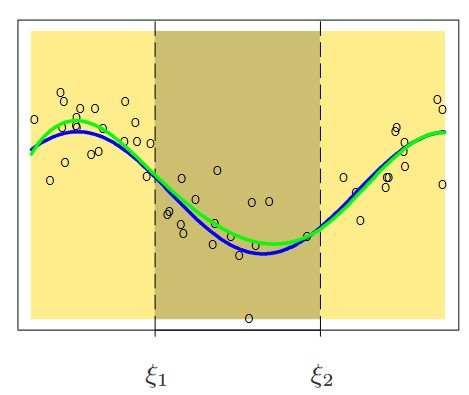
\includegraphics[width=\textwidth,height=0.6\textheight]{spline_visual.jpg}
\caption{A cubic spline function with 2 knots (courtesy of Hastie,
Tibshirani, and Friedman (2009))}
\end{figure}
\end{column}
\end{columns}

We defer more information about spline functions to Wood (2017)

We assume the knots of the functions are equidistance.
\end{frame}

\begin{frame}{Generalized Additive Models with Splines}
\protect\hypertarget{generalized-additive-models-with-splines}{}
\textbf{Generalized additive model} (Hastie and Tibshirani 1987) is
expressed \begin{align*}
  y_i &\simiid EF(\mu_i, \phi), \quad i = 1, \dots, n\\
  g(\mu_i) &= \beta_0 + B(x_i) = \beta_0 + \bs X_i^T \bs \beta ,  \quad \mathbb{E}\left[B(X)\right] = 0 
\end{align*} where \(B(x_i)\) is the spline function, \(g(\cdot)\) is a
link function, \(\phi\) is the dispersion parameter

\vspace*{0.5cm}

\begin{itemize}
\tightlist
\item
  Model fitting follows the generalized linear models, e.g.~ordinary
  least square for Gaussian outcome \[
  \boldsymbol{\hat \beta} = \text{arg}\min \sum\limits^n_{i=1} \left[y_i - \beta_0 - \bs X_i^T \bs \beta \right]^2
  \]
\end{itemize}
\end{frame}

\begin{frame}{Problem: Function Smoothness}
\protect\hypertarget{problem-function-smoothness}{}
The estimation of \(B(X)\) can be wiggly when the underlying function is
smooth, particularly as the number of bases ,\(K\), increases.

{[}TODO: add two plots, overfitting and not overfitting{]}
\end{frame}

\hypertarget{bayesian-regularization}{%
\subsection{Bayesian Regularization}\label{bayesian-regularization}}

\begin{frame}{Smoothing Spline Model}
\protect\hypertarget{smoothing-spline-model}{}
\begin{itemize}
\item
  Smoothing penalty
  \(\lambda \int B^{''}(X)^2dx = \lambda \bs \beta^T \bs S \bs\beta\)

  \begin{itemize}
  \tightlist
  \item
    The smoothing penalty matrix \(\bs S\) is known given \(\bs X\)
  \item
    \(\bs S\) is symmetric and positive semi-definite
  \end{itemize}
\item
  Penalized Least Square for Gaussian Outcome \[
  \boldsymbol{\hat \beta} = \text{arg}\min \sum\limits^n_{i=1} \sum\limits^n_{i=1} \left[y_i - \beta_0 - \bs X_i^T \bs \beta \right]^2 + \lambda \bs \beta^T \bs S \bs\beta
  \]
\item
  The smoothing parameter \(\lambda\) is a tuning parameter, selected
  via cross-validation
\end{itemize}
\end{frame}

\begin{frame}{Problem: Multiple Predictor Model}
\protect\hypertarget{problem-multiple-predictor-model}{}
When a model contains multiple spline functions for variables
\(X_1, \dots, X_p\), the penalized least square estimator is \[
\boldsymbol{\hat \beta} = \text{arg}\min \sum\limits^n_{i=1} \sum\limits^n_{i=1} \left[y_i - \beta_0 - \sum\limits \bs X_{ij}^T \bs \beta_j \right]^2 + \lambda_j \bs \beta_j^T \bs S_j \bs\beta_j
\]

\emph{How to decide \(\lambda_i\)?}

\begin{itemize}
\tightlist
\item
  Global smoothing, i.e.~\(\lambda_1 = \cdots =\lambda_p\) assumes all
  functions shares the same shape
\item
  Adaptive smoothing, i.e.~examining \(\lambda_i\) combination, are
  computationally intensive
\end{itemize}
\end{frame}

\begin{frame}{Bayesian Regularization}
\protect\hypertarget{bayesian-regularization-1}{}
\begin{itemize}
\tightlist
\item
  Bayesian Regularization is the Bayesian analogy of penalized models by
  using regularizing priors

  \begin{itemize}
  \tightlist
  \item
    Bayesian ridge via normal prior \[
     \beta \sim N(0, \tau^2) \rightarrow  \lambda = \sigma^2/\tau^2
    \]
  \end{itemize}
\item
  Adaptive shrinkage with hierarchical priors \[
   \tau^2_j \simiid IG(a, b)
  \]

  \begin{itemize}
  \tightlist
  \item
    Adaptive Smoothing

    \begin{itemize}
    \tightlist
    \item
      Random walk prior on b-spline bases with IG hyperprior
    \item
      Normal prior on truncated power bases with a log-normal spline
      model for variance
    \end{itemize}
  \end{itemize}
\end{itemize}
\end{frame}

\hypertarget{bayesian-variable-selection}{%
\subsection{Bayesian Variable
Selection}\label{bayesian-variable-selection}}

\begin{frame}{Problem: Functional Selection}
\protect\hypertarget{problem-functional-selection}{}
In the context of variable selection and high-dimensional statistics, we
always assume some variables are not effective or predictive to the
outcome.

How to statistically detect

\begin{itemize}
\tightlist
\item
  if a variable is predictive to the outcome, \(B_j(X_j) = 0\)
\item
  if a variable has a nonlinear relationship with the outcome,
  \(B_j(X_j) = \beta_j X_j\)
\end{itemize}

\emph{Bi-level selection} is the procedure that simultaneously addresses
the two questions above
\end{frame}

\begin{frame}{Spike-and-Slab Priors}
\protect\hypertarget{spike-and-slab-priors}{}
Spike-and-slab priors are a family of mixture distributions that deploys
a characterizing structure
\[\beta|\gamma \sim (1-\gamma)f_{spike}(\beta) + \gamma f_{slab}(\beta)\]

\begin{itemize}
\item
  Latent indicator \(\gamma\) follows a Bernoulli distribution with
  probability \(\theta\)
\item
  Spike density \(f_{spike}(x)\) concentrates around 0 for small effects
\item
  Slab density \(f_{slab}(x)\) is a flat density for large effects
\item
  Natural procedure to select variables via posterior distribution of
  \(\gamma\)
\item
  Markov chain Monte Carlo is not compelling for high-dimensional data
  analysis
\end{itemize}
\end{frame}

\begin{frame}{Spike-and-Slab LASSO Priors}
\protect\hypertarget{spike-and-slab-lasso-priors}{}
\begin{itemize}
\tightlist
\item
  Double exponential distributions as the spike and slab distributions
  \[\beta|\gamma \sim (1-\gamma)DE(0, s_0) + \gamma DE(0, s_1), 0 < s_0 < s_1\]

  \begin{itemize}
  \tightlist
  \item
    Seamless variable selection as coefficients shrinkage to 0
  \item
    Computation advantages via Expectation-Maximization (EM) algorithms
  \end{itemize}
\item
  Group spike-and-slab LASSO

  \begin{itemize}
  \tightlist
  \item
    Structure underlying predictors, e.g.~gene pathways, bases of a
    spline function
  \item
    Structured prior on \(\gamma\) \[
    \gamma_k | \theta_j ~ Binomial(1, \theta_j), k \in j
    \]
  \end{itemize}
\end{itemize}
\end{frame}

\begin{frame}{Problem: High-dimensional Spline Model}
\protect\hypertarget{problem-high-dimensional-spline-model}{}
How to jointly model signal sparsity and function smoothness, while
capable of bi-level selection?

\begin{itemize}
\tightlist
\item
  Excess shrinkage due to ignoring smooth penalty completely

  \begin{itemize}
  \tightlist
  \item
    Group lasso penalty (Ravikumar et al. 2009; Huang, Horowitz, and Wei
    2010), group SCAD penalty (Wang, Chen, and Li 2007; Xue 2009)
  \item
    Global penalty VS adaptive penalty
  \end{itemize}
\item
  All-in-all-out selection

  \begin{itemize}
  \tightlist
  \item
    Can not detect if a function is linear, e.g.~spike-and-slab grouped
    LASSO prior (Bai et al. 2020; Bai 2021)
  \item
    Failed to select function as whole, e.g.~group spike-and-slab LASSO
    prior
  \end{itemize}
\item
  Computational prohibitive algorithms

  \begin{itemize}
  \tightlist
  \item
    MCMC algorithms doesn't scale well for high-dimensional models
    (Scheipl, Fahrmeir, and Kneib 2012)
  \end{itemize}
\end{itemize}
\end{frame}

\hypertarget{dissertation}{%
\section{Dissertation}\label{dissertation}}

\begin{frame}{Objectives}
\protect\hypertarget{objectives}{}
\begin{itemize}
\tightlist
\item
  To develop statistical models that improve curve interpolation and
  outcome prediction

  \begin{itemize}
  \tightlist
  \item
    Local adaption of sparse penalty and smooth penalty
  \item
    Bi-level selection for linear and nonlinear effect
  \end{itemize}
\item
  To develop a fast and scalable algorithm
\item
  To implement a user-friendly statistical software
\end{itemize}
\end{frame}

\begin{frame}[fragile]{Scope}
\protect\hypertarget{scope}{}
Scope of this dissertation * BHAM * Survival Model * R package
\texttt{BHAM}
\end{frame}

\hypertarget{references}{%
\section*{References}\label{references}}
\addcontentsline{toc}{section}{References}

\begin{frame}[allowframebreaks]{References}
\hypertarget{refs}{}
\begin{CSLReferences}{1}{0}
\leavevmode\vadjust pre{\hypertarget{ref-Bai2021}{}}%
Bai, Ray. 2021. {``Spike-and-Slab Group Lasso for Consistent Estimation
and Variable Selection in Non-Gaussian Generalized Additive Models.''}
\emph{arXiv:2007.07021v5.}

\leavevmode\vadjust pre{\hypertarget{ref-Bai2020}{}}%
Bai, Ray, Gemma E Moran, Joseph L Antonelli, Yong Chen, and Mary R
Boland. 2020. {``Spike-and-Slab Group Lassos for Grouped Regression and
Sparse Generalized Additive Models.''} \emph{Journal of the American
Statistical Association}, 1--14.

\leavevmode\vadjust pre{\hypertarget{ref-Hastie1987}{}}%
Hastie, Trevor, and Robert Tibshirani. 1987. {``{Generalized additive
models: Some applications}.''} \emph{Journal of the American Statistical
Association} 82 (398): 371--86.
\url{https://doi.org/10.1080/01621459.1987.10478440}.

\leavevmode\vadjust pre{\hypertarget{ref-hastie2009elements}{}}%
Hastie, Trevor, Robert Tibshirani, and Jerome Friedman. 2009. \emph{The
Elements of Statistical Learning: Data Mining, Inference, and
Prediction}. Springer Science \& Business Media.

\leavevmode\vadjust pre{\hypertarget{ref-Huang2010}{}}%
Huang, Jian, Joel L Horowitz, and Fengrong Wei. 2010. {``Variable
Selection in Nonparametric Additive Models.''} \emph{Annals of
Statistics} 38 (4): 2282.

\leavevmode\vadjust pre{\hypertarget{ref-Ravikumar2009}{}}%
Ravikumar, Pradeep, John Lafferty, Han Liu, and Larry Wasserman. 2009.
{``{Sparse additive models}.''} \emph{Journal of the Royal Statistical
Society: Series B (Statistical Methodology)} 71 (5): 1009--30.
\url{https://doi.org/10.1111/j.1467-9868.2009.00718.x}.

\leavevmode\vadjust pre{\hypertarget{ref-Scheipl2012}{}}%
Scheipl, Fabian, Ludwig Fahrmeir, and Thomas Kneib. 2012.
{``{Spike-and-slab priors for function selection in structured additive
regression models}.''} \emph{Journal of the American Statistical
Association} 107 (500): 1518--32.
\url{https://doi.org/10.1080/01621459.2012.737742}.

\leavevmode\vadjust pre{\hypertarget{ref-Wang2007}{}}%
Wang, Lifeng, Guang Chen, and Hongzhe Li. 2007. {``Group SCAD Regression
Analysis for Microarray Time Course Gene Expression Data.''}
\emph{Bioinformatics} 23 (12): 1486--94.

\leavevmode\vadjust pre{\hypertarget{ref-Wood2017}{}}%
Wood, Simon N. 2017. \emph{{Generalized additive models: An introduction
with R, second edition}}. \url{https://doi.org/10.1201/9781315370279}.

\leavevmode\vadjust pre{\hypertarget{ref-Xue2009}{}}%
Xue, Lan. 2009. {``Consistent Variable Selection in Additive Models.''}
\emph{Statistica Sinica}, 1281--96.

\end{CSLReferences}
\end{frame}

\end{document}
